% !TEX root = sum1.tex

\section{Results}
% The nested structure makes the greedy method useful.
% Remark: Similar to what we mentioned, the greedy method refers to using the largest groups to fill the seats.

We carried out several experiments, including comparing the running time of decomposition and Integer programming, comparing the number of people served using the feasible seat planning and Integer programming methods, analyzing different policies under the two booking situations, investigating the impact of seat layout on the number of served people, evaluating the results under varying demands, and finally assessing the results for different numbers of people in each period.


% Improvement:
% For $\X^{0}$, we introduce one empty seat, $x_1$. But it cannot provide the feasibility.

% \subsection{Deterministic Model}\label{Deterministic_result}
% The integer programming \eqref{deter_upper} can be solved quickly because of the monotone ratio.


\subsection{Running time of Benders Decomposition and IP}\label{Bender_IP}

% In view of the fact that IP of the deterministic model can be solved quickly, the column generation method does not show an obvious advantage. 

% At first, we compare the running time of these two methods. 

The running times of solving IP directly and using Benders decomposition are shown in Table \ref{tab_1}. 

\begin{table}[ht]
  \centering
  \caption{Running time of Decomposion and IP}\label{tab_1}
  \begin{tabular}{|l|l|l|l|l|l|l|}
  \hline
  \# of scenarios & demands & running time of IP(s) & Benders (s) & \# of rows & \# of groups & \# of seats\\
  \hline
  1000  & (150, 350) & 5.1  & 0.13 & 30 & 8 & (21, 50)\\
  5000  & & 28.73 & 0.47 & 30 & 8 \\
  10000 & & 66.81  & 0.91 & 30 & 8 \\
  50000 & & 925.17 & 4.3 & 30 & 8 \\
  \hline
  1000  & (1000, 2000) & 5.88 & 0.29 & 200 & 8 & (21, 50)\\
  5000  & & 30.0 & 0.62 & 200 & 8 \\
  10000 & & 64.41 & 1.09 & 200 & 8 \\
  50000 & & 365.57 & 4.56 & 200 & 8 \\
  \hline
  1000  & (150, 250) & 17.15  & 0.18 & 30 & 16 & (41, 60) \\
  5000  & & 105.2  & 0.67 & 30 & 16  \\
  10000 & & 260.88 & 1.28 & 30 & 16  \\
  50000 & & 3873.16 & 6.18 & 30 & 16  \\
  \hline
  \end{tabular}
\end{table}

The parameters in the columns of the table are the number of scenarios, the range of demands, running time of integer programming, running time of Benders decomposition method, the number of rows, the number of group types and the number of seats for each row, respectively. 

Take the first experiment as an example, the scenarios of demands are generated from (150, 350) randomly, the number of seats for each row is generated from (21, 50) randomly.
% about 1000 seats.

% The second one:
% The number of seats for each row L is generated from (21, 50) randomly, about 7000 seats.
% The scenarios of demands are generated from (1000, 2000) randomly.

% The third one:
% The number of seats for each row L is generated from 41-60 randomly, about 1500 seats.
% The scenarios of demands are generated from (150, 250) randomly.


\subsection{Feasible Seat Planning versus IP Solution}

A arrival sequence can be expressed as $\{y_{1}, y_{2}, \ldots, y_{T}\}$. Let $N_{j} = \sum_{t} I(y_t = j)$, i.e., the count number of times group type $j$ arrives during $T$ periods. Then the scenarios, $(N_1, \ldots, N_{J})$, follow a multinomial distribution, $$p\left(N_1, \ldots, N_{J} \mid \mathbf{p}\right)=\frac{T !}{N_{1}!, \ldots, N_{J}!} \prod_{j=1}^{J} p_{j}^{N_j}, T = \sum_{j=1}^{J} N_{j}.$$

It is clear that the number of different sequences is $J^{T}$. The number of different scenarios is $O(T^{J-1})$ which can be obtained by the following DP.

Use $D(T,J) $ to denote the number of scenarios, which equals the number of different solutions to $x_{1}+\ldots + x_{J} = T, \mathbf{x} \geq 0$. Then, we know the recurrence relation $D(T, J) = \sum_{i= 0}^{T} D(i, J-1)$ and boundary condition, $D(i,1) = 1$. So we have $D(T,2) = T+1$, $D(T,3) = \frac{(T+2)(T+1)}{2}, D(T,J) = O(T^{J-1})$. 

The number of scenarios is too large to enumerate all possible cases. Thus, we choose to sample some sequences from the multinomial distribution.

Then, we will show the near-optimal seat assignment has a close performance with IP when considering nested policy.

% Then we compare the results of benders decomposition and IP under nested policy.

\begin{table}[ht]
    \caption{Results of Decomposion and IP under nested policy}
    \begin{tabular}{|l|l|l|l|l|l|}
    \hline
    \# samples & T & probabilities & \# rows & people served by decomposition & people served by IP \\
    1000  & 45  & [0.4,0.4,0.1,0.1] & 8 & 85.30 & 85.3 \\
    1000  & 50  & [0.4,0.4,0.1,0.1] & 8 & 97.32 & 97.32 \\
    1000  & 55  & [0.4,0.4,0.1,0.1] & 8 & 102.40 & 102.40  \\ % slow
    1000  & 60  & [0.4,0.4,0.1,0.1] & 8 & 106.70 & NA  \\
    1000  & 65  & [0.4,0.4,0.1,0.1] & 8 & 108.84 & 108.84 \\
    \hline
    1000  & 35  & [0.25,0.25,0.25,0.25] & 8 & 87.16 & 87.08 \\
    1000  & 40  & [0.25,0.25,0.25,0.25] & 8 & 101.32 & 101.24 \\
    1000  & 45  & [0.25,0.25,0.25,0.25] & 8 & 110.62 & 110.52 \\
    1000  & 50  & [0.25,0.25,0.25,0.25] & 8 & 115.46 & NA \\
    1000  & 55  & [0.25,0.25,0.25,0.25] & 8 & 117.06 & 117.26 \\
    \hline
    5000  & 300  & [0.25,0.25,0.25,0.25] & 30 & 749.76 & 749.76 \\
    5000  & 350  & [0.25,0.25,0.25,0.25] & 30 & 866.02 & 866.42 \\
    5000  & 400  & [0.25,0.25,0.25,0.25] & 30 & 889.02 & 889.44 \\
    5000  & 450  & [0.25,0.25,0.25,0.25] & 30 & 916.16 & 916.66 \\
    \hline
    \end{tabular}
\end{table}

Each entry of people served is the average of 50 instances.
IP will spend more than 2 hours in some instances, as `NA' showed in the table.
The number of seats is 20 when the number of rows is 8, the number of seats is 40 when the number of rows is 30.

We can find that the people served by Benders decomposition and IP under nested policy are close. But obtaining the near-optimal seat assignment will be faster.

% Thus, we can use the near-optimal seat assignment from the decomposition approach.

\subsection{Results of Different Policies}

We present the results of policies compared to the optimal policy.

For seat assignment after booking period, we have DSA.

DP and FCFS-based are for seat assignment during booking period.

\begin{table}[ht]
  \centering
  \caption{Results of Policies}
  \begin{tabular}{|l|l|l|l|l|l|l|}
  \hline
   T & probabilities & \# of rows & DSA(\%) & Row by Row(\%) & DP(\%) & FCFS-based(\%) \\
  \hline
   60  & [0.45 0.05 0.05 0.45] & 10 & 98.24 & 97.39 & 99.49 & 99.08 \\
   60  & [0.35 0.05 0.35 0.25] & 10 & 98.12 & 97.93 & 99.62 & 99.25 \\
   60  & [0.25 0.05 0.65 0.05] & 10 & 98.55 & 97.91 & 99.39 & 99.28 \\ % slow
   60  & [0.35 0.15 0.15 0.35] & 10 & 97.28 & 98.14 & 99.29 & 99.12 \\
   60  & [0.25 0.15 0.45 0.15] & 10 & 96.30 & 97.59 & 99.46 & 99.09 \\
  \hline
  \end{tabular}
\end{table}


\subsection{Result of Different Demands}

In this subsection, we discuss the effect of the number of periods on the results of our experiments. Specifically, we consider two situations: c = 2.5 and c = 1.9.

When c = 2.5, we set the parameters as follows: T = 10-100, step size = 1, expected number of periods = 60, expected number of demand (people) = 150, number of rows = 10, and number of seats per row = 21.

When c = 1.9, we set the parameters as follows: T = 30-120, step size = 1, expected number of periods = 72, expected number of demand (people) = 137, number of rows = 10, and number of seats per row = 21.

For each $c$, we give several probabilities in the table. The gap point represents the first period where the number of people without social distancing is larger than that with social distancing and the gap percentage is the corresponding percentage of total seats.


% We can find that the difference between the number of accepted people and the number of total people will increase with the period. 


\begin{table}[ht]
  \centering
  \caption{Gap points of different probabilities}
  \begin{tabular}{|l|l|l|l|}
  \hline
  c  & probabilities & gap point & gap percentage \\
  \hline
  2.5  & [0.25,0.25,0.25,0.25] & 56 & 65.21 \\
  2.5  & [0.1,0.4,0.4,0.1] & 55 & 65.59 \\
  2.5  & [0.1, 0.5, 0.2, 0.2] & 55 & 65.45 \\
  2.5  & [0.2, 0.3, 0.3, 0.2] & 54 & 64.56 \\
  2.5  & [0.3, 0.2, 0.2, 0.3] & 55 & 65.51\\
  2.5  & [0.2, 0.4, 0.1, 0.3] & 55 & 65.41 \\
  1.9  & [0.4, 0.4, 0.1, 0.1] & 67 & 60.35 \\
  1.9  & [0.5, 0.2, 0.2, 0.1] & 67 & 58.9  \\
  1.9  & [0.3, 0.5, 0.2, 0]  &  68 & 61.7  \\
  1.9  & [0.6, 0.1, 0.1, 0.2] & 66 & 58.31 \\
  \hline
  \end{tabular}
\end{table}


We provide the results of our experiments for people accepted when applying social distance and not applying social distance over different periods. The different probabilities with the same $c$ share the similar pattern of the figure, so we only provide one case to show the detailed figure.


\begin{figure}[h]
  \centering
  \subfigure[When $c =2.5$]{
    \label{Fig.sub.1}
    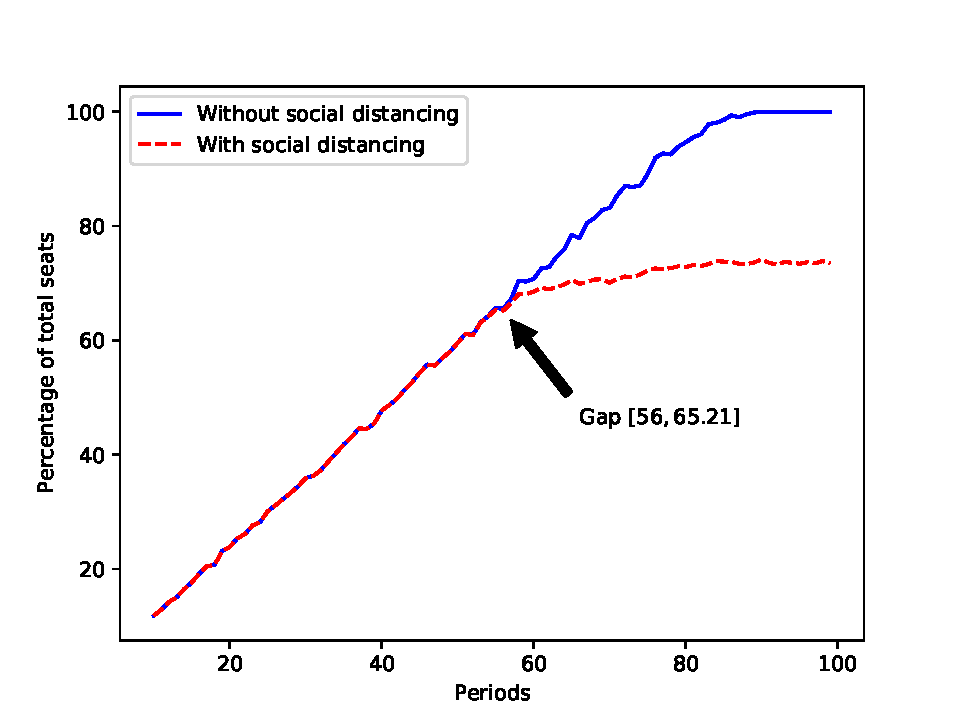
\includegraphics[width=0.48\textwidth]{./Figures/p1.pdf}}
  \subfigure[When $c =1.9$]{
    \label{Fig.sub.2}
    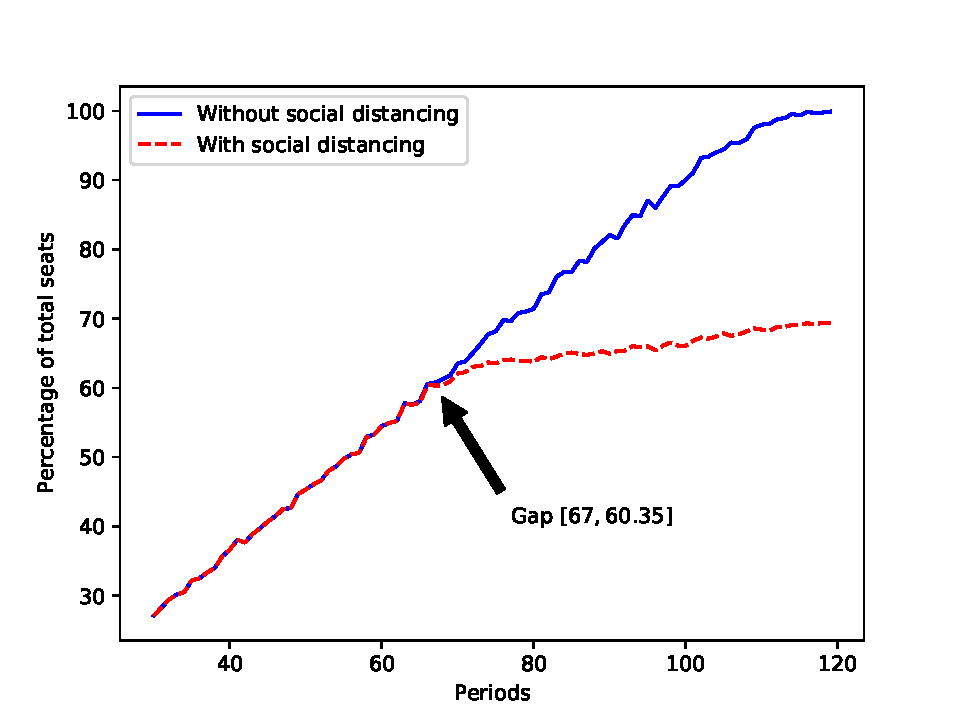
\includegraphics[width=0.48\textwidth]{./Figures/p2.pdf}}
  \caption{The number of people served versus periods}
  \label{Fig.lable}
\end{figure}


There are three stages, the first stage is when the capacity is sufficient. The measure of social distancing will not cause any effect. The gap is becoming larger as $T$ increases at the second stage. At the third stage, as $T$ continues to increase, the gap will converge when the capacity is limited.

We can estimate the attendance rate from $\frac{c}{c+1}*$ the number of seats. The number of periods will be $E(D)/c$. Thus, the government can make the policy on how much attendance rate can be established.


\subsection{Results of Different Arriving People Per Period}

In this subsection, we discuss the effect of different probabilities on our experimental results. Assuming that groups of up to four people can sit together, we calculate the expected number of demands as $E(D) = (p_1 * 1 + p_2 * 2 + p_3 * 3 + p_4 * 4) T$, where $p_1$, $p_2$, $p_3$, and $p_4$ represent the probabilities of groups with one, two, three, and four people, respectively. We also define $c = p_1 * 1 + p_2 * 2 + p_3 * 3 + p_4 * 4$ and choose $T(E(D)/c)$ such that the supply is near the demand. We then compare the number of people served under different values of $c$.


% Different $T$ has little effect on the number of people served using M6 because it is based on first-come-first-served. 

We sample $p_1$, $p_2$, and $p_3$ from 0.05 to 0.95 with an increment of 0.05. We call each realization $(p_1, p_2, p_3, p_4)$ the probability combination when $p_1 + p_2 + p_3 + p_4 = 1$.
The number of all sampled probability combinations is $n_p$. The number of rows is set at 10, and the number of seats per row is 21 (including one dummy seat). We simulate 200 periods, and the number of people served with respect to the value of $c$ is shown in the figure below. For each probability combination, the blue point represents the average number of people served from 50 instances and the red point represents the expected number of people served.


% \begin{figure}[h]
%   \centering
%   \subfigure[One instance for each data point]{
%     \label{Fig.sub.1}
%     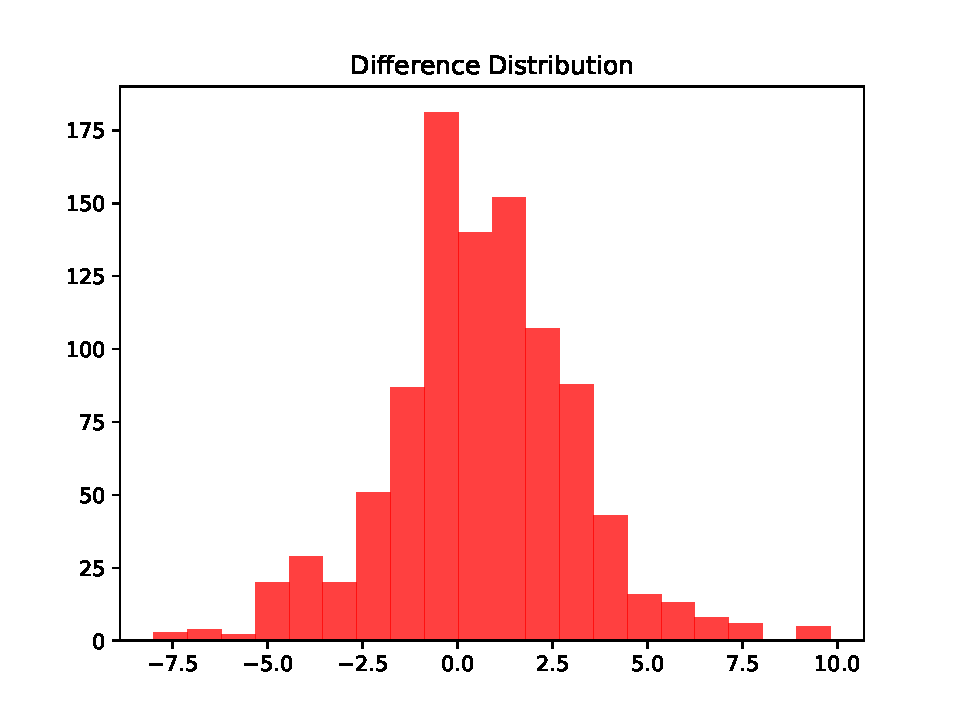
\includegraphics[width=0.48\textwidth]{./Figures/Figure_1.pdf}}
%   \subfigure[Average of 50 instances for each data point]{
%     \label{Fig.sub.2}
%     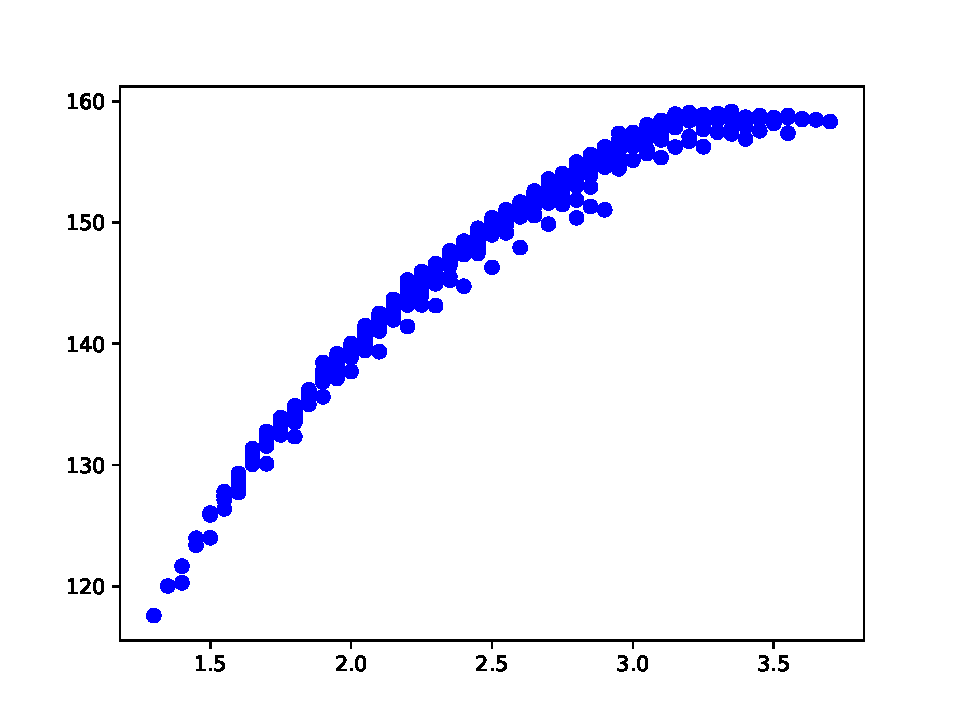
\includegraphics[width=0.48\textwidth]{./Figures/Figure_2.pdf}}
%   \caption{The number of people served versus $c$}
%   \label{Fig.lable}
% \end{figure}

% \begin{figure}[ht]
%   \centering
%   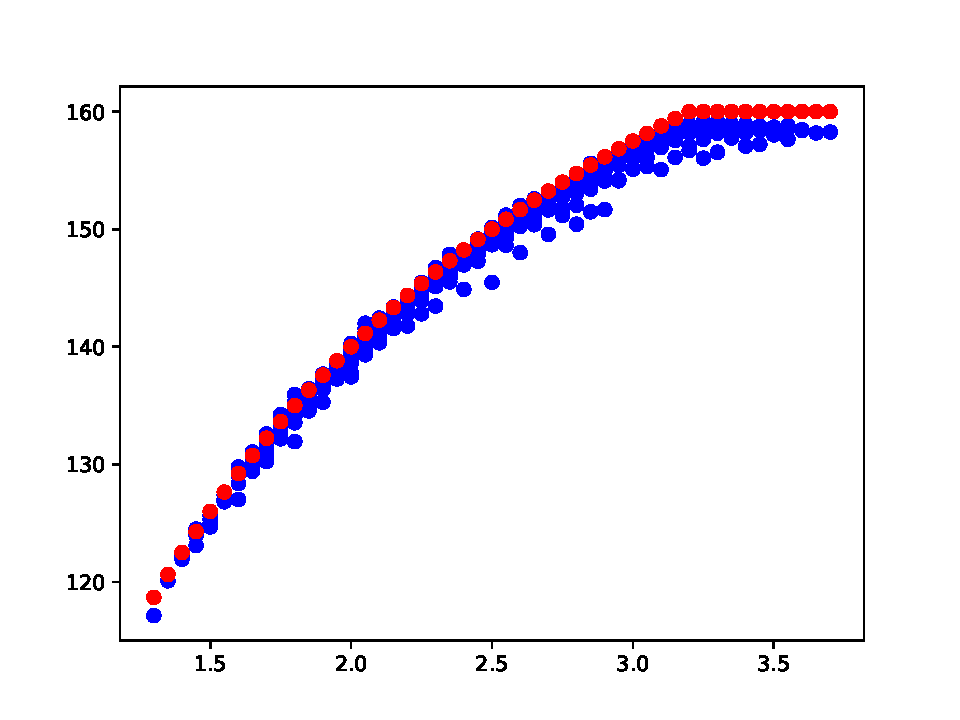
\includegraphics[width = 0.7\textwidth]{./Figures/diff_2.pdf}
%   \caption{The number of people served versus $c$}
% \end{figure}

\begin{figure}[h]
  \centering
  \subfigure[One instance for each probability combination]{
    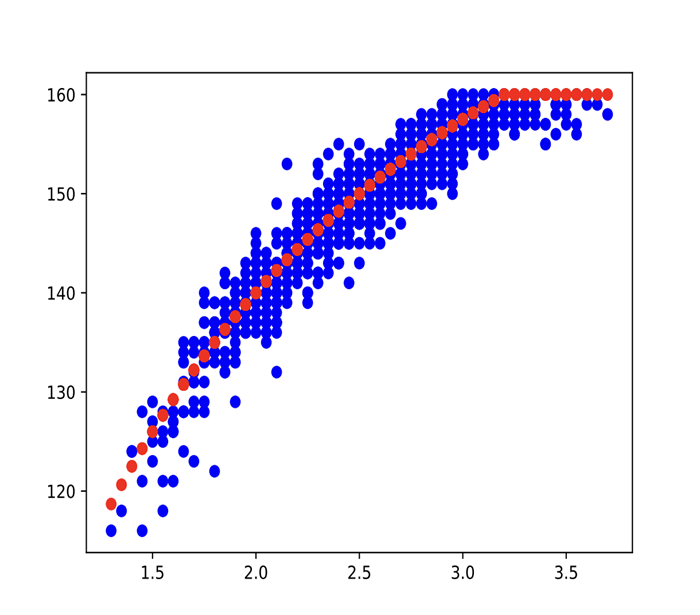
\includegraphics[width=0.48\textwidth]{./Figures/diff_1.jpg}}
  \subfigure[Average of 50 instances for each probability combination]{
    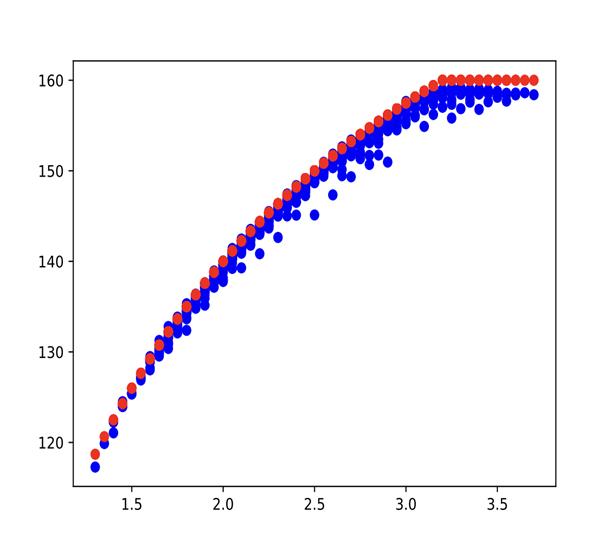
\includegraphics[width=0.48\textwidth]{./Figures/diff_2.jpg}}
  \caption{The number of people served versus $c$}
\end{figure}

Suppose we accept $D_a$ people with $T$ arrivals, where $D_a = c * T$, and the sum of $D_a$ and $T$ is equal to the total number of seats. In this case, the estimation of the occupancy rate is $\frac{c}{c+1}$. The number of people served is near $\frac{c}{c+1} * 210$ on average (as shown by the red points in the figure).

% when there are full patterns for all rows.

If the largest pattern is assigned for each row, the occupancy rate is $\frac{16}{21}$. The maximum number of people that can be served is $210 * \frac{16}{21} = 160$, which is the upper bound of the number of people served.

We also observe that some blue points are far from the red points in the figure. For example, when the probability is $[0.05, 0.05, 0.85, 0.05] (c = 2.9)$, the demands can be $[4, 1, 45, 2]$ or $[2, 2, 47, 1]$. It is not possible to construct all full patterns for every row with these demands, violating our assumption and resulting in a large gap between the blue and red points in this case.


% When $p = [0.25, 0.25, 0.25, 0.25]$, $E(D) = 2.5 T$. Let $p_1*1 + p_2*2 + p_3*3 + p_4*4 = 2.5$, 
% Let $E(D) = 150, T = 50, 60, 75$. The number of seats: 200, 210, 225.

% 1: When $E(D)$ is fixed, case3,4 need a larger hall to accept the same number of people.

% Different layout may make a difference.

% 2. The assumption that $T$ is fixed will be more reasonable for the continuous time. 

We can give the absolute difference between the blue point and red point for each probability combination as below.

\begin{table}[ht]
  \centering
  \caption{Difference Distribution}
  \begin{tabular}{|l|l|l|l|l|}
  \hline
  \# of instances & abs\_diff $\geq$ 1 & abs\_diff $\geq$ 2 & abs\_diff $\geq$ 3 & abs\_diff $\geq$ 4 \\
  \hline
  20 & 32.92 \% & 5.13 \% & 1.74\% & 0.51 \% \\
  50 & 22.46 \% & 4.31 \% & 1.54 \% & 0.31 \%  \\
  100 & 20.00 \% & 4.21 \% & 1.54 \% & 0.31 \% \\
  \hline
  \end{tabular}
\end{table}


\begin{figure}[ht]
  \centering
  \subfigure[Average of 50 instances for each probability combination]{
    \label{Fig1}
    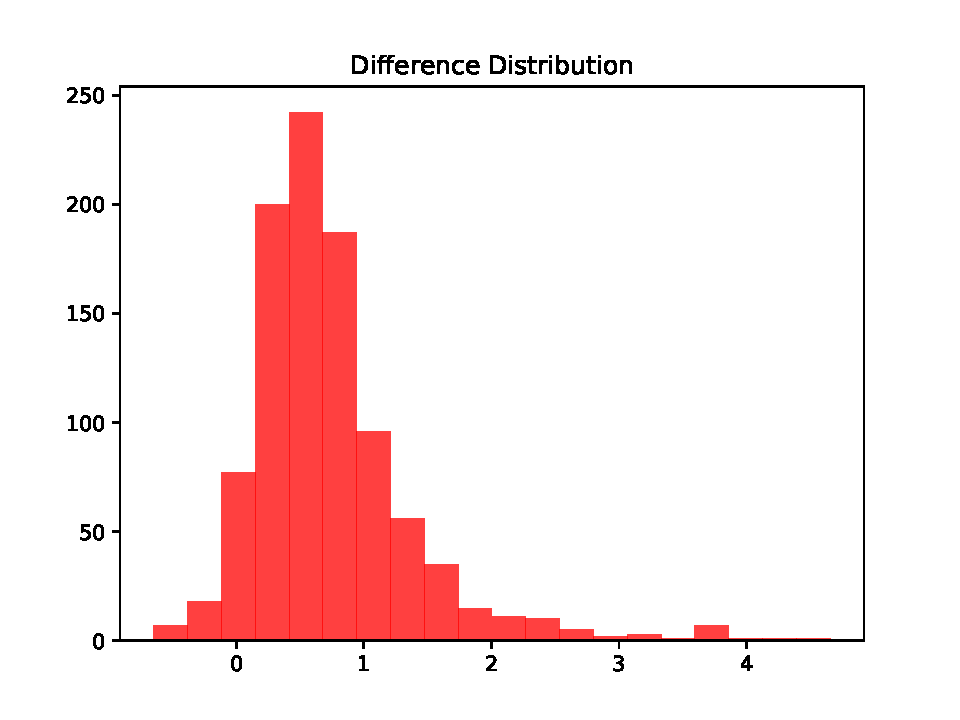
\includegraphics[width=0.48\textwidth]{./Figures/Figure_50.pdf}}
  \subfigure[Average of 100 instances for each probability combination]{
    \label{Fig2}
    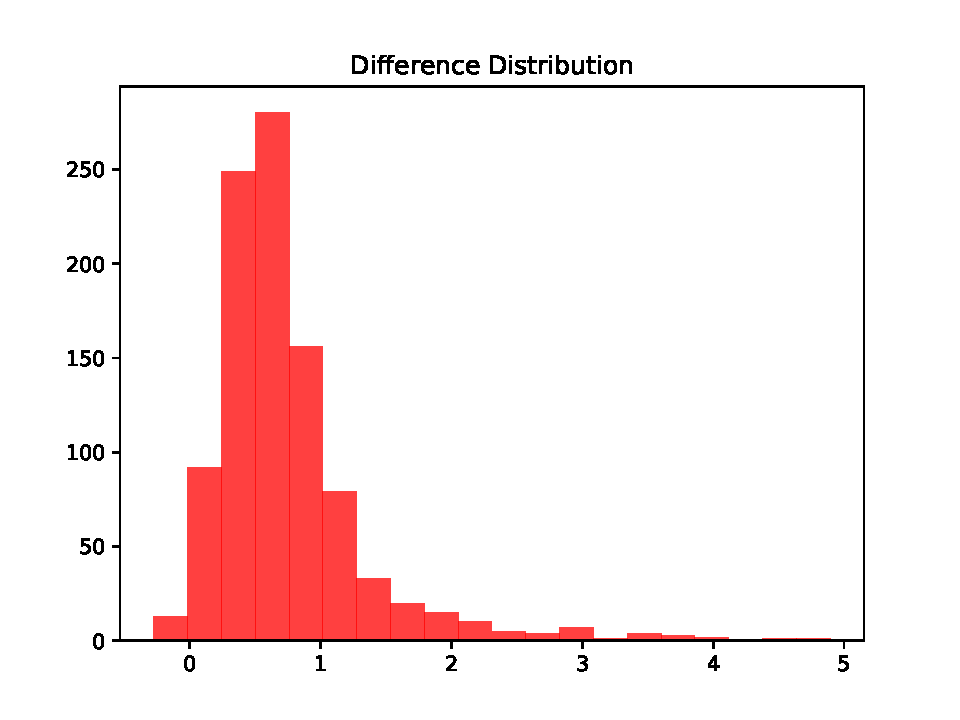
\includegraphics[width=0.48\textwidth]{./Figures/Figure_100.pdf}}
  \caption{The difference distribution}
  \label{Fig}
\end{figure}

The results show that we can estimate attendance rate based on $c$ for most probability combinations. 


\subsection{Seat Layout}

The number of seats are $[17,18,19,20,21,21,22,23,24,25]$. The maximal number of people that can be served is 164.

Random seat layout: $[26, 21, 24, 20, 20, 17, 23, 19, 21, 19]$. The maximal number of people that can be served is 164.

\begin{figure}[ht]
  \centering
  \subfigure[Average of 50 instances for step-size seat layout]{
    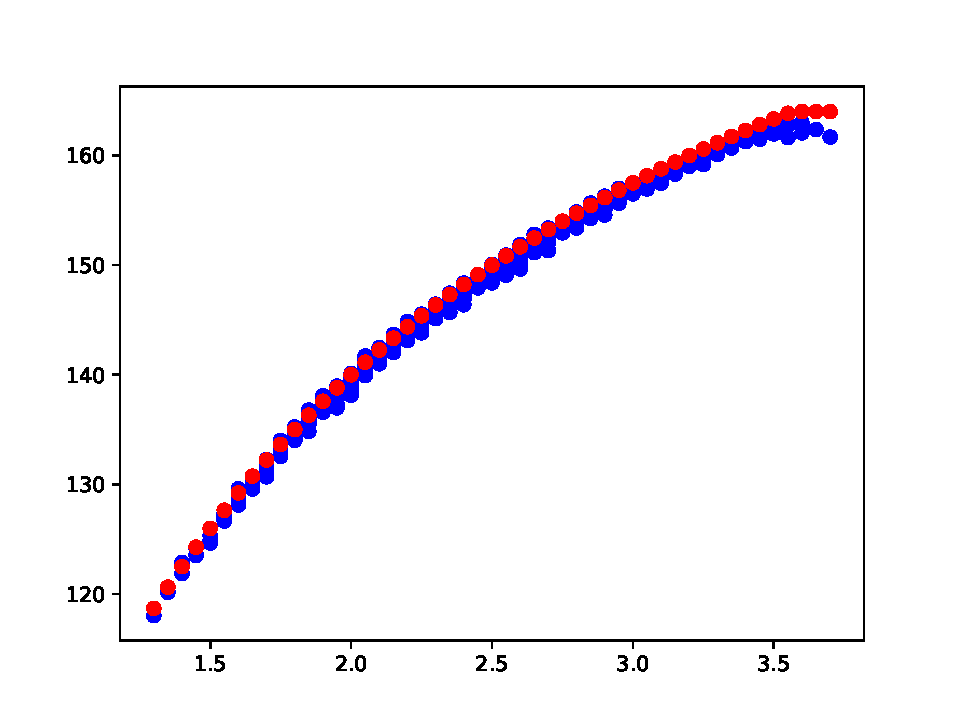
\includegraphics[width=0.48\textwidth]{./Figures/stepsize_seat.pdf}}
  \subfigure[Average of 50 instances for random seat layout]{
    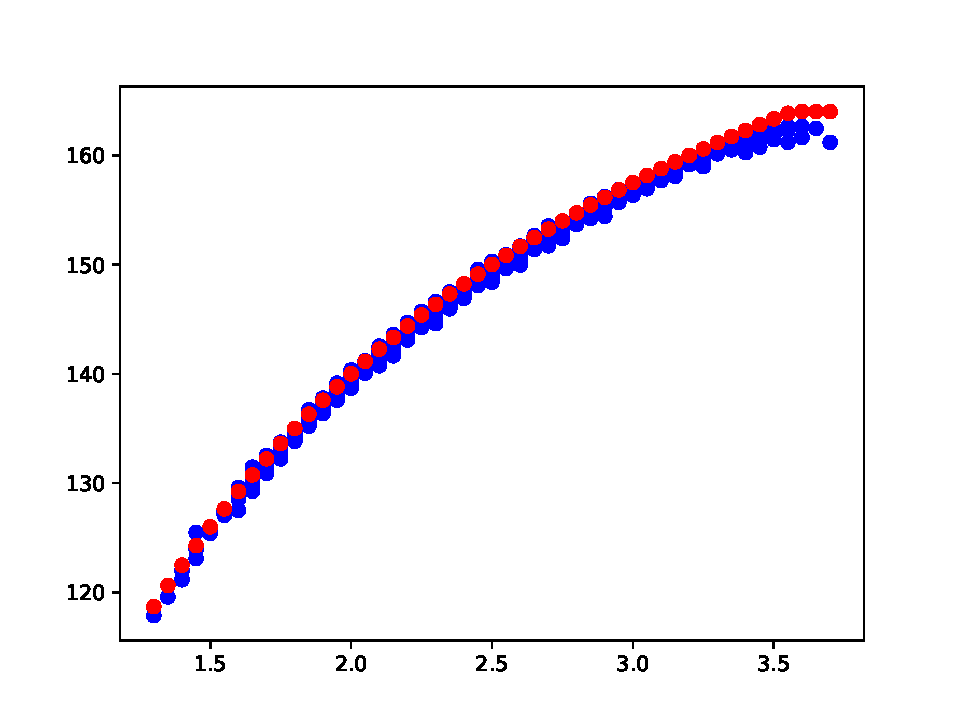
\includegraphics[width=0.48\textwidth]{./Figures/random_seat.pdf}}
  \caption{The number of people served versus $c$}
\end{figure}


\newpage


% \subsection{Group of Different Sizes}
% Let $c$ be $2.5$ for groups of different sizes.

% Probability of group size of 3: $[0.1, 0.3, 0.6]$.

% Probability of group size of 5: $[0.3, 0.3, 0.1, 0.2, 0.1]$.

% \begin{figure}[h]
%   \centering
%   \subfigure[group size of 3]{
%     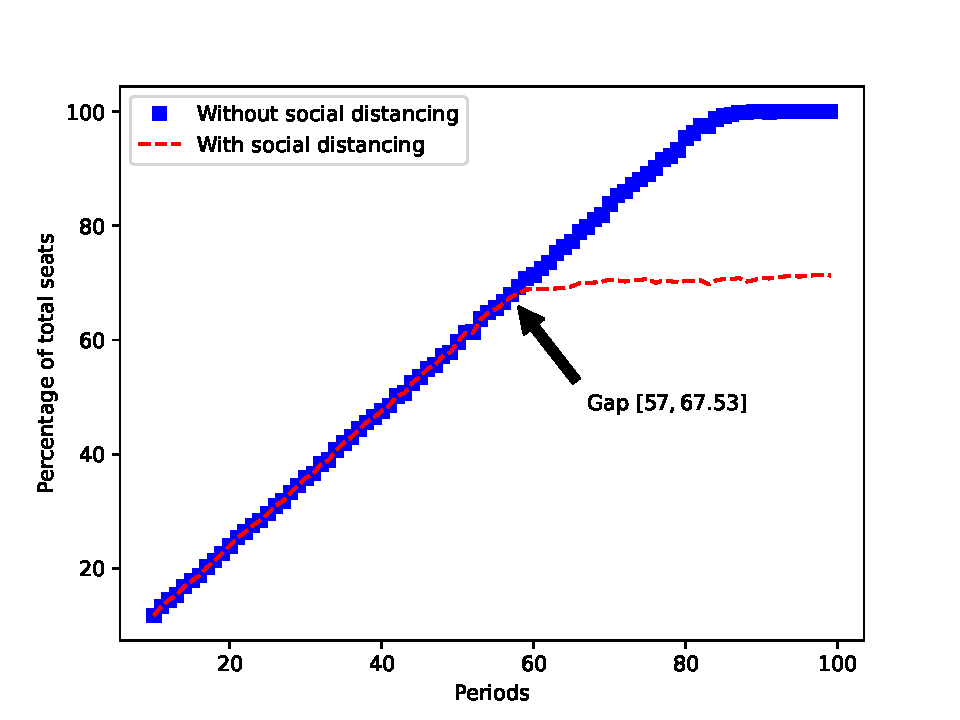
\includegraphics[width=0.48\textwidth]{./Figures/group3.pdf}}
%   \subfigure[group size of 5]{
%     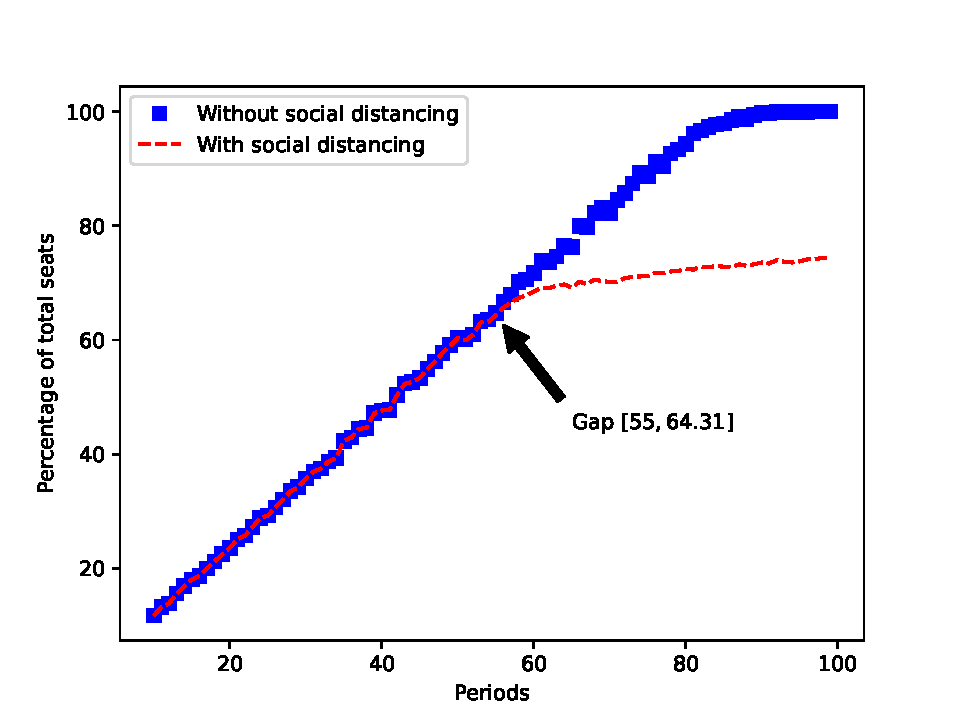
\includegraphics[width=0.48\textwidth]{./Figures/group5.pdf}}
%   \caption{The number of people served versus periods}
% \end{figure}

% \subsection{Measurement}

% Suppose a real scenario with a fixed sequence, $s^{r}$. Solving the following program can obtain the optimal value, $V_{s^{r}}$. (Offline)

% Then the difference is $V_{s^{r}} - \text{our result}$.

% WS(the value under wait-and-see policy with all possible scenarios)

% EVPI(Expected Value of Perfect Information) = WS - the value of deterministic equivalent form

% Regret.

% Several things need to do:

% What is greedy result like?

% Why does period run so slowly?

% Revise lemma

% lack of the traits


\newpage
